\chapter{Ontwerp van het project}
\label{hoofdstuk:ontwerp}

Eenmaal de belangrijkste vereisten gekend zijn kan er een ontwerp opgetekend worden. Daarom even de grote lijnen die te concluderen vallen uit hoofdstuk \ref{hoofdstuk:doelen}:

\begin{itemize}
  \item De data en het visuele aspect van de applicatie moeten zo ontkoppeld mogelijk zijn, elk moet apart uitbreidbaar zijn
  \item Zeer grote hoeveelheden data moeten vlot kunnen behandeld en genavigeerd worden: zoeken, filteren, sorteren, aanpassen, \ldots
  \item De data moet zowel centraal als decentraal toegankelijk zijn en synchronisatie toestaan
  \item Compatibiliteit met de reeds geschreven onderdelen van het project moet indien mogelijk bewaard blijven
  \item Om het ontwerp te verifi\"eren moet een werkend programma gemaakt worden, gebruiksvriendelijkheid, functionaliteit en snelheid zijn hierbij belangrijk
\end{itemize}

\section{De grote lijnen}
Van alle vereisten die rechtstreeks invloed kunnen uitoefenen op de architectuur, is de splitsing van de data en de visualisatie waarschijnlijk de meest fundamentele. Een beproefde aanpak om dit te realizeren is het ontwerppatroon genaamd \emph{Model-View-Controller (MVC)}\footnote{Een algemeen overzicht kan men bijvoorbeeld bekomen op \url{http://en.wikipedia.org/wiki/Model-view-controller}}.\\

Het doel is een ontwerp te maken waarin we een visualisatiemethode kunnen verbinden aan de juiste databron. Enkele zaken moeten echter nog vastgelegd worden, namelijk: wat is de basiseenheid van data? Waar zal een visualisatiemodule achter vragen? Zoals in figuur~\ref{fig:flow} te zien is, ligt de focus bij dit project op koppelingen van fragmenten in plaats van fragmenten op zich. Er zijn op het eerste zicht twee alternatieven om dit te modelleren. De eerste mogelijkheid is een soort van \emph{MatchedFragment} die een fragment beschrijft plus een lijst met alle fragmenten die er potentieel aan gekoppeld kunnen worden en op welke locatie. De tweede mogelijkheid is om elk paar een apart object te laten voorstellen (bvb. genaamd \emph{FragmentPair}). Het eerste alternatief lijkt het voordeel te hebben dat het gemakkelijk is om na te kijken of een fragment reeds ``bezet'' is. Ook zou het dan mogelijk zijn om bijvoorbeeld een grafe op te stellen door van brokstuk naar brokstuk te springen. Echter, dit soort opstelling bevat op het eerste zicht veel redundantie, een fragment zal op die manier een verwijzing met attributen naar een fragment bevatten, en dit fragment zal op zijn beurt een identieke omgekeerde verbinding hebben. De redundantie vermijden en een verwijzing als een apart object voorstellen waar beide fragmenten naar kunnen verwijzen is eigenlijk niets anders dan de tweede optie (een \emph{FragmentPair}). Op die manier wordt de situatie omgedraaid en kan een fragmentenpaar verwijzen naar de fragmenten die het opbouwen. Daarbij kan het probleem van hoe de ``bezetting'' van een object te weten te komen (alsook de grafe, zoals later zal aangetoond worden) opgelost worden door de vereiste zoekfunctionaliteit van het datamodel te benutten.\\

Eenmaal de basiseenheid van informatie gekozen is, valt de kern van de applicatie volgens MVC uit te beelden als in figuur~\ref{fig:basicprogramflow}.

\begin{figure}[ht]
	\begin{center}
		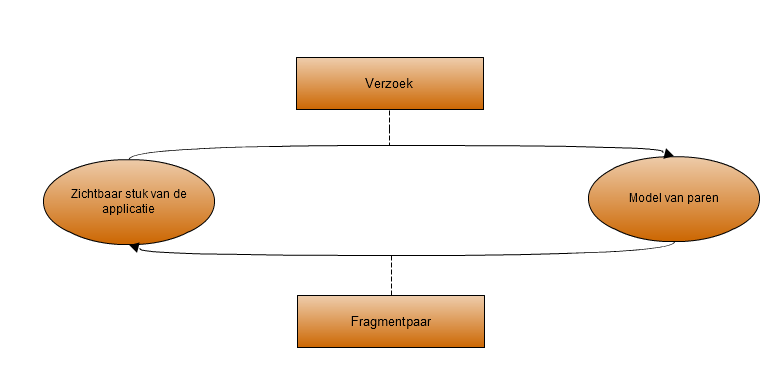
\includegraphics[width=1.0\columnwidth]{images/BasicExecutionFlow.png}
		\caption{Het abstracte model van de applicatie, links staat de \emph{View/Controller} en rechts het \emph{Model}. De controller stuurt een verzoek naar het model voor een bepaalde (sub)set van de data --- al dan niet gesorteerd --- en het model antwoord met alle paren die voldoen aan de criteria}
		\label{fig:basicprogramflow}
	\end{center}
\end{figure}

\subsection{Modellen}

\ldots Elk model heeft een selectie die ook gedeeld kan worden

\subsection{Verzoeken}

\subsubsection{Opvragen}
Het concept achter het opvragen van fragmentparen is dat er steeds wordt begonnen vanuit de volledige beschikbare verzameling. Deze kan dan \textbf{gereduceerd} en \textbf{gesorteerd} worden. \\

Sorteren is eenvoudig en kan op eender welk attribuut in stijgende of dalende zin gebeuren. Filters gebruiken een simpele maar krachtige syntax die volledig gelijk is aan die van de \emph{WHERE}-clausule van een SQL zin (voorbeeld: broncode~\ref{code:sortingfiltering}). Geavanceerde gebruikers kunnen op deze manier zelf filters verzinnen, veelgebruikte filters en sorteeroperaties kunnen echter best als knoppen en invoervelden blootgesteld worden, zoals in figuur~\ref{fig:tangfiltersort}.\\

De voorwaarde die aan filters gesteld wordt is dat ze enkel attributen beschrijven die werkelijk bestaan, filters die naar een onbestaand attibuut refereren worden genegeerd.\\

Er kunnen meerdere filters op een model actief zijn, deze werken dan conjunctief. Op die manier kunnen meerdere modellen filters plaatsen zonder met elkaar in conflict te komen. 

\lstinputlisting[language=C++,label=code:sortingfiltering,caption=Een voorbeeld van hoe een model kan gebruikt worden in een applicatie]{source/sortingfiltering.cpp}

\begin{figure}[ht]
  \centering
  \subfloat[Sorteren]{
    \label{fig:tangsorting}
    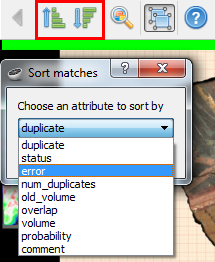
\includegraphics[width=0.30\textwidth]{images/tangerine-sorting.png}
  }\hfill%%%%%%%%%%%%%%%%%%%%%% <========
  \subfloat[Filteren op namen van fragmenten]{
    \label{fig:tangfiltering}
    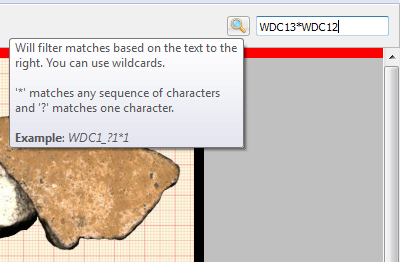
\includegraphics[width=0.60\textwidth]{images/tangerine-namefilter.png}
  }
  \caption{Basis sorteer- en filteroperaties worden via de gebruikersinterface blootgesteld}
  \label{fig:tangfiltersort}
\end{figure}

% \begin{figure}[ht]
%   \begin{minipage}{0.30\textwidth}
%     \centering
%     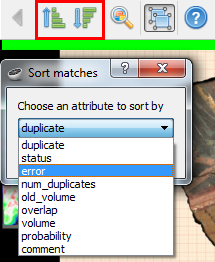
\includegraphics[width=0.60\textwidth]{images/tangerine-sorting.png}
% 	\caption{Sorteren}
% 	\label{fig:tangsorting}
%   \end{minipage}\hfill
%   \begin{minipage}{0.60\textwidth}
%     \centering
%     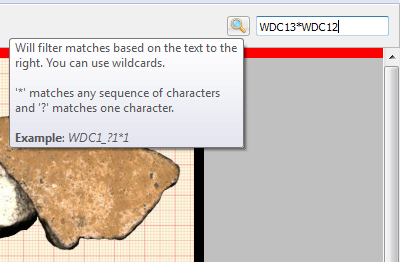
\includegraphics[width=0.60\textwidth]{images/tangerine-namefilter.png}
% 	\caption{Filteren op de namen van de fragmenten}
% 	\label{fig:tangfiltering}
%   \end{minipage}\hfill
% \end{figure}

\subsubsection{Aanpassingen}
Veranderingen aan de inhoud van de database 
Een verzoek\ldots

Er zijn twee grote klassen
Er kan gesorteerd worden op attributen en er kan gefilterd worden o

\subsection{Fragmentenparen}
Het zoeken naar de gewenste verzameling van paren gebeurt via een verzoek en wordt aan het model overgelaten, maar wat kan een component doen met de paren die dan ter beschikking komen? Op zijn minst bestaat een paar uit twee fragmenten en een resem eigenschappen. Die eigenschappen of attributen kunnen gaan van een maatstaf voor de fout toegekend door de automatische herkenner, tot de validatie die een onderzoeker aan het voorstel heeft gegeven. De objecten die geproduceerd worden door de automatische paarherkenners van het theraproject voldoen aan deze twee voorwaarden. Er bestaan reeds veel componenten die hiervan gebruik maken dus dezelfde interface recycleren zou de integratie van het project een heel deel vergemakkelijken. Alle aanpassingen die zich niet kunnen beperken tot \'e\'en paar kunnen via het model afgehandeld worden.\\

\section{Modulariteit}
Om het geheel uitbreidbaar te maken is een pluginsysteem gemaakt. Er is een hoofdapplicatie (codenaam ``Tangerine'') die de connectie maakt met de databeheerlaag en verschillende visualisatieplugins kan laden. Het basissysteem zonder modules bestaat uit een manier om een fragmenten en paren-database in te laden en te kiezen welke module op te starten.\\

De eerste en meest uitgewerkte daarvan werd \emph{MatchTileView} gedoopt. Het geeft de paren op dezelfde manier weer als het Browsematches prototype, maar is natuurlijk uitgebreid qua mogelijkheiden. De bespreking van de toegevoegde functionaliteiten komt aan het bod in het hoofdstuk over modules.\\

\begin{figure}[ht]
	\begin{center}
		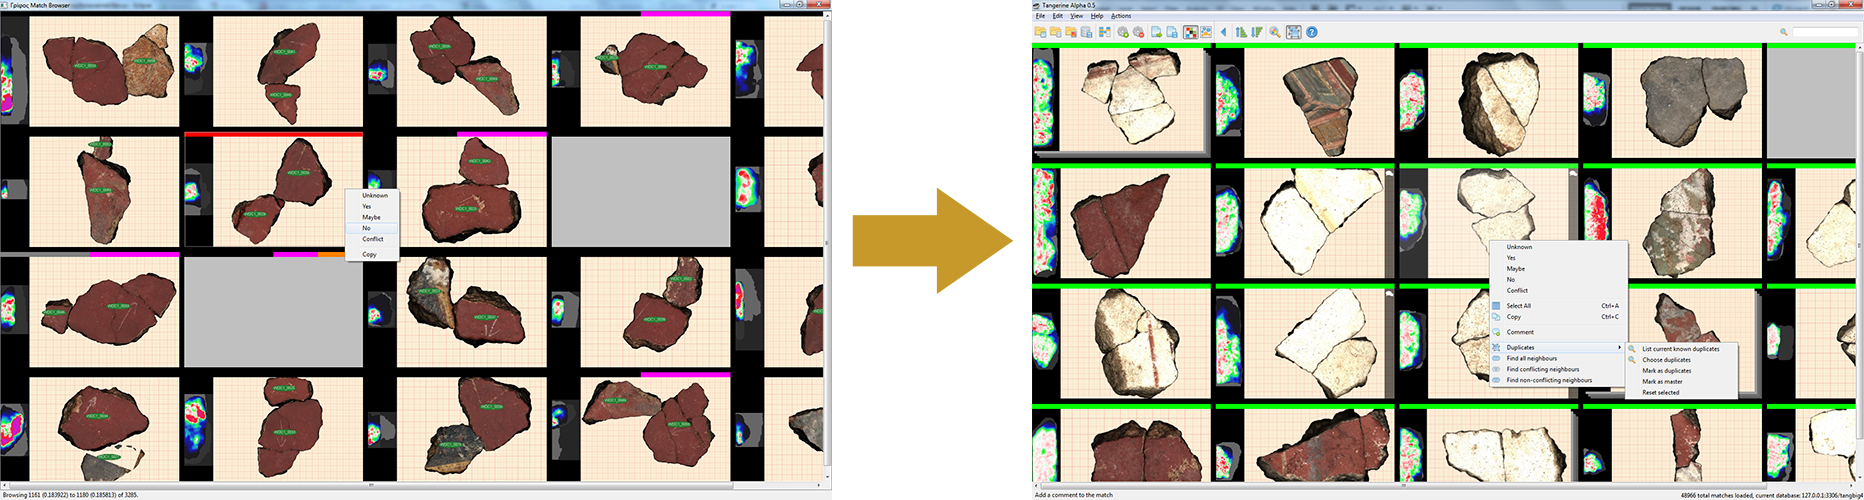
\includegraphics[width=1.0\columnwidth]{images/browsematches-to-tangerine-01.png}
		\caption{De manier van weergeven uit Browsematches werd gekopi\"eerd naar het nieuwe platform, met uitbreidingen}
		\label{fig:browsematchestotang}
	\end{center}
\end{figure}

Elke module krijgt van de applicatie een model toegewezen waar het fragmentparen uit kan opvragen. Dit kan een nieuw model zijn zonder criteria of een gedeeld model. Een gedeeld model behoort niet exclusief tot een module en betekent bijvoorbeeld dat als er \'e\'en beslist om te sorteren op een attribuut zoals ``het verschil van de dikte tussen twee fragmenten'', alle modules die gebruikmaken van ditzelfde model opeens over een gesorteerde dataset beschikken. Via speciale signalen worden zij hiervan op de hoogte gebracht, zodat ze kunnen beslissen of het nodig is een actie te ondernemen. Dit kan handig zijn voor pure visualisatieplugins die geen zoekmogelijkheden aan de gebruiker blootstellen, het kan dan vertrouwen op andere modules om data aan te leveren.\\

Indirecte communicatie via het model is (voorlopig) de enige manier waarop modules elkaar kunnen be\"invloeden. De structuur van de componenten ziet er uit als in figuur~\ref{fig:visualizationlayer}. Merk op dat er een plugin is (\emph{DetailView}) die geen gebruik maakt van fragmentparen maar eerder van een virtueel tafelblad net als Griphos. Zoals eerder aangehaald kunnen fragmentparen automatisch op een tafelblad gezet worden. Dit tafelblad kan dan in 3D weergegeven worden door \emph{DetailView}, waarover later meer.

\begin{figure}[h]
	\begin{center}
		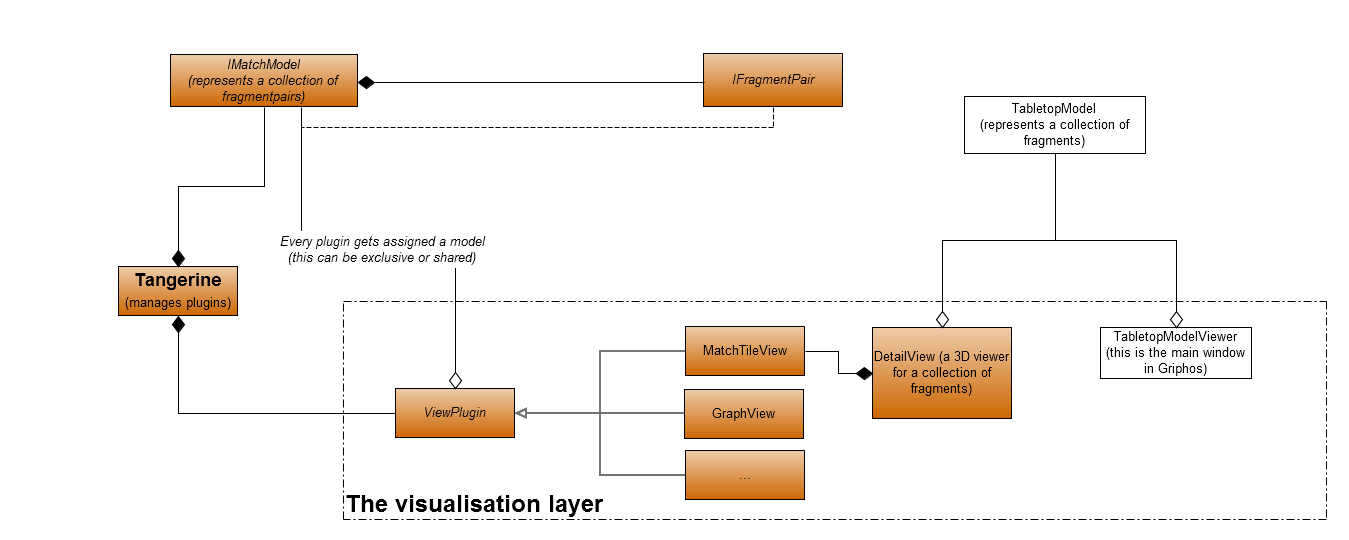
\includegraphics[width=1.0\columnwidth]{images/VisualizationExtract.png}
		\caption{Een vereenvoudigde kijk op de componenten van de visualisatielaag, het hoofdscherm en het model. De componenten in het wit behoren tot de rest van het thera project en zijn niet gemaakt als deel van dit thesisproject.}
		\label{fig:visualizationlayer}
	\end{center}
\end{figure}

\section{Dataoplsag, synchronizatie, \ldots}
De oplossing om aan de vereisten van centrale en decentrale toegang, grote hoeveelheden data en navigatie te voldoen wordt in hoodstuk \ref{hoofdstuk:database} besproken. Het is echter reeds duidelijk dat er een database zal moeten gebruikt worden. Om twee van deze databases te verenigen is er een component ontwikkeld die een aantal fasen doorloopt. De mogelijkheid bestaat om er later nog meer te maken maar voorlopig zijn er 3 fasen: \textbf{Gebruikers}, \textbf{Paren} en \textbf{Attributen}. In elke fase krijgt de gebruiker een scherm te zien met de verschillen tussen de 2 databases die een algoritme heeft gedetecteerd en krijgt ze de mogelijkheid om aanpassingen te maken alvorens naar de volgende fase over te stappen. Het is belangrijk gebruikers keuzes te laten maken waarin ze ge\"interesseerd zijn en ze niet lastig te vallen met keuzes die ze niet willen maken (beide zaken negeren leidt tot frustraties~\cite{Joel2001}). Het algoritme probeert steeds een standaardkeuze in te vullen aan de hand van heuristieken (dit hangt af van de fase), de gebruiker kan deze indien gewenst natuurlijk veranderen. Tegelijkertijd moet de gebruiker ge\"informeerd worden van alle stappen die het algoritme zal ondernemen. 

\subsection{Paren}

Overeenkomsten met verschillende id
Overeenkomsten met dezelfde id
Conflicten met dezelfde id
Geen conflict, geen overeenkomst

Deze subcomponent laat aan de volgende fasen weten welke acties er zijn ondernomen, meer bepaald welke id-transformatie een bepaalde object heeft meegemaakt

\subsection{Attributen}
\subsection{Geschiedenis}

\section{Gebruiksgemak / visuele interface}
De gebruikersinterface en de achterliggende bibliotheken werden gemaakt met behulp van de Qt toolkit~\cite{qtdoc}

Vergelijking van wachttijden tussen Griphos/Browsematches en Tangerine

Geheugengebruik BM na grote db: 350 MB (geen afbeeldingen)

Griphos: tonen van een lijst met aparte fragmenten om uit te kiezen (geen equivalent in BM/Tang)
Griphos: tonen van een lijst met alle paren (zoals te zien in figuur~\ldots): 7 minuten 18 seconden <--- NOOT: Griphos gebruikt dezelfde manier van fragmenten inladen als Browsematches, maar laadt ook op voorhand alle afbeeldingen in. Het geheugengebruik na het openenen van 49471 paren is 1.5 GB RAM, het heropenen van dit scherm neemt evenveel tijd in beslag. Het lijkt erop dat het geheugen niet vrijgemaakt noch herbruikt wordt, want bij de tweede keer moest het besturingssysteem het programma afsluiten wegens te veel geheugengebruik.
Browsematches: opstarten en een lijst van alle paren tonen: 49471 paren = 160 seconden en 350MB
Thesisproject: 

\rowcolors{2}{gray!50}{white}
\begin{center}
	\begin{tabular}{|l|r|r|r|}
	    \rowcolor{gray!75}
	    \hline
	    & \textbf{Griphos} &  \textbf{Browsematches} & \textbf{Thesis (MySQL)} \\
	    \hline
	    \textbf{Opstartsnelheid} & 1 sec & 16 sec & 1 sec \\
	    \textbf{Fragmenten inladen} & 1 min 35 sec  & - & - \\
	    \textbf{\textasciitilde 4000 paren laden} & - & 16 sec & 0 sec \\
	    \textbf{\textasciitilde 50000 paren laden} & 7 min 18 sec & 2 min 47 sec  & 0-3 sec* \\
	    \textbf{\textasciitilde 250000 paren laden} & niet getest & niet getest & 0-15 sec* \\
	    \hline
	\end{tabular}
\end{center}

* Deze getallen zijn afhankelijk van de cache die op de moment aanwezig is, enige vorm van recente activiteit op de database zal ervoor zorgen dat de responstijd rond de 100 milliseconden ligt. De reden dat het soms lang duurt is omdat het programma vraagt achter het totaal aantal fragmenten, en dit is voor de geteste types van databases geen snelle operatie (alles moet geteld worden). Het cijfer verchilt ook per type database

Alle informatie die alleenstaande brokstukken toebehoort --- naam, 3D-voorstelling, contour, \ldots --- wordt opgeslagen als een grote verzameling mappen in het bestandssysteem. Hoewel niet alles meteen wordt ingeladen neemt dit soms toch wat tijd in beslag. Hetzelfde geldt voor een collectie paarvoorstellen waarvan een eerste scherm moet ingeladen worden. Weer een andere bron van vertraging bij het opstarten is het inladen van alle modules, vooral degene die gebruikmaken van OpenGL om fragmenten in 3D weer te geven. Deze stappen  Om deze reden is er voor gezorgd dat deze operaties parallel kunnen lopen, zodat de gebruiker zo weinig mogelijk moet wachten en steeds informatie kan krijgen over de vooruitgang.

De gemiddelde opstarttijd voor Browsematches gemeten op een AMD Athlon X2 5600+ met 2 GB RAM is 10 seconden, waardoor de gebruiker reeds snel gaat denken dat er iets misgelopen is. Bij Browsematches duurde het bijvoorbeeld  is nog  een. 

Alle modules kunnen acties zoals knoppen en menu's  Elk programma dat Bij het initialiseren 

% DATA
\section{Het beheer van de data}

Redenering: Alles vloeit voort uit de paren, het is voorspelbaar (simpel voor te stellen) en ondubbelzinnig

Het zelf kunnen maken van paren is van secundair belang (volgens de thesis), zij kunnen door de HumanMatcher ingevoerd worden in de grote database

Griphos is zeer nuttig -> identificatie locatie van fragmenten in de bak, etc. -> Tangerine is het ontbrekende middendeel!

Dit betekent echter niet dat beide perspectieven elkaar uitsluiten, integendeeel.
 
[TODO: verhuizen naar ontwerp van database]

% VISUALISATIE
\section{Visualisatie, een manier om met de data te werken}

\subsection{Model-View-Controller}

\subsection{UML diagramma}

[maak UML diagramma]\\

\section{Integratie in thera project}
Gebruik van bibliotheken, ...
Extensie door refactoring: FragmentConf -> IFragmentConf ==> SQLFragmentConf | FragmentConf
Hierdoor is het nodig om de reeds bestaande code van het thera project om te zetten naar het gebruik van IFragmentConf waar mogelijk maar het aanmaken van FragmentConf anderzijds
of FragmentConf ==> SQLFragmentConf
Alternatieve oplossing, geen veranderingen in thera code maar SQLFragmentConf sleept dan veel onnodige ballast mee van FragmentConf

\section{Uitbreidbaarheid}
[afbeeldingen invoegen]\\


[afbeelding invoegen, selectie naar grafe transit!]\\